\section{Experiments}
\label{sec:experiments}



\subsection{Benchmarks}
We evaluate PivotRL on the following agentic benchmarks:
\begin{itemize}
  \item \textbf{$\tau^2$-bench} \citep{barres2025tau2bench} focuses on conversational tool-use in a multi-turn customer service setting. It contains 3 subsets: Retail and Airline \citep{yao2024taubench}, which tests agent tool-calling, and Telecom, which adds the complexity of user tool-calls. We keep the user model fixed to \texttt{Qwen3-235B-A22B-Instruct-2507} across our evaluations.
  \item \textbf{Terminal-Bench} \citep{tbench_2025} evaluates the model on bash terminal-use tasks that range from filesystem navigation, coding, and system administration to complex problem-solving scenarios such as training machine learning models, configuring legacy systems, and reverse engineering binary files. We evaluate on the TBCore-v1.1 set of questions using the Terminus-2 harness.
  \item \textbf{Swe-Bench} \citep{jimenez2024swebench} evaluates the model on various real-world programming tasks that can be described as understanding an issue, localizing the issue in a codebase, and creating a code patch to resolve the issue. We use the SWE-Bench-Verified subset which is a widely adopted set of 500 verifiable questions. We evaluate using the OpenHands harness. 
  \item \textbf{BrowseComp}
  \citep{wei2025browsecompsimplechallengingbenchmark} tests the search agent capabilities of a model through very difficult questions that require critical reasoning and the use of a search engine to answer correctly. It often results in very long trajectories with many search calls for each problem, and is shown to be a hard benchmark for current frontier LLMs.
\end{itemize}

\begin{table}[!t]
\centering
\small
\begin{tabular}{lcccc}
\toprule
\textbf{Benchmark} & \textbf{Qwen3-30B (\%)} & SFT & \textbf{PivotRL (\%)} & \textbf{Gain ($\Delta$)} \\ 
\midrule
$\tau^2$-Bench     & 44.35 & & 63.81 & +19.46 \\
SWE-Verified       & 19.07 & & 32.67 & +13.6 \\
Terminal-Bench     & 5.42  & & 20.00 & +14.58 \\ 
BrowseComp         & 2.50  & & 11.30 & +8.80  \\
\bottomrule
\end{tabular}
\caption{Main results of benchmark accuracy gain after training with PivotRL on \texttt{Qwen3-30B-A3B-Thinking-2507}.}
\label{tab:main_results_enhanced}
\end{table}
% \begin{table}[!t]
% \centering
% \small % Slightly smaller font to ensure it fits well in double-column layouts
% \resizebox{\linewidth}{!}{%
% \begin{tabular}{l c cc cc cc cc}
% \toprule
% \multirow{2}{*}{\textbf{Benchmark}} & \textbf{Baseline} & \multicolumn{2}{c}{$\tau^2$-\textbf{Bench}} & \multicolumn{2}{c}{\textbf{SWE-Verified}} & \multicolumn{2}{c}{\textbf{Terminal-Bench}} & \multicolumn{2}{c}{\textbf{BrowseComp}} \\
% \cmidrule(lr){3-4} \cmidrule(lr){5-6} \cmidrule(lr){7-8} \cmidrule(lr){9-10}
% & \textbf{Qwen3-30B} & \textbf{sft} & \textbf{rl} & \textbf{sft} & \textbf{rl} & \textbf{sft} & \textbf{rl} & \textbf{sft} & \textbf{rl} \\
% \midrule
% IFBench        & 52.04 & 44.42 & 53.29 & - & 51.72 & 24.77 & 49.47 & 54.35 & 53.89 \\
% AIME25         & 86.04 & 76.25 & 85.63 & - & 84.58 & 21.56 & 82.92 & 85.21 & 85.83 \\
% MATH500        & 98.05 & 98.00 & 98.35 & - & 98.00 & 63.55 & 98.00 & 98.30 & 98.40 \\
% LiveCodeBench  & 66.52 & 64.98 & 66.96 & - & 67.62 & 45.15 & 64.54 & 67.62 & 66.96 \\
% Scicode (subtask) & 36.83 & 31.95 & 38.68 & - & 36.39 & 9.39  & 39.13 & 35.58 & 37.28 \\
% MMLU-Pro       & 80.84 & 79.81 & 81.31 & - & 80.70 & 71.57 & 80.85 & 81.13 & 81.31 \\
% MMLU-ProX      & 78.58 & 74.31 & 78.92 & - & 78.55 & 59.13 & 78.49 & 76.68 & 78.60 \\
% WMT24++ (en$\rightarrow$xx)       & 36.97 & 34.25 & 36.54 & - & 36.71 & 6.31  & 36.48 & 33.18 & 36.26 \\
% \bottomrule
% \end{tabular}%
% }
% \caption{Out-of-domain regression analysis results after training with PivotRL on \texttt{Qwen3-30B-A3B-Thinking-2507}. No SFT was done on the SWE-Bench targeted model due to using non-thinking data for PivotRL.}
% \label{tab:main_results_regression}
% \end{table}

\begin{table*}[!t]
\centering
\small
\resizebox{\textwidth}{!}{%
\begin{tabular}{l c cc cc cc cc}
\toprule
\multirow{3}{*}{\textbf{Benchmark}} 
& \multirow{3}{*}{\textbf{Baseline}} 
& \multicolumn{8}{c}{\textbf{Training Domain (score + $\Delta$)}} \\
\cmidrule(lr){3-10}
& 
& \multicolumn{2}{c}{$\tau^2$} 
& \multicolumn{2}{c}{SWE} 
& \multicolumn{2}{c}{Terminal} 
& \multicolumn{2}{c}{BrowseComp} \\
\cmidrule(lr){3-4} \cmidrule(lr){5-6} \cmidrule(lr){7-8} \cmidrule(lr){9-10}
& Qwen3-30B 
& sft & rl 
& sft & rl 
& sft & rl 
& sft & rl \\
\midrule
\midrule

\textbf{Peak In-Domain} 
& -- 
& 58.44 (+14.09) & 63.81 (+19.46)
& 37.40 (+18.33) & 32.67 (+13.60)
& 13.75 (+8.33)  & 20.00 (+14.58)
& 1.50 (-1.00)   & 11.30 (+8.80) \\
\midrule

IFBench 
& 52.04 
& 44.42 (-7.62) & 53.29 (+1.25)
& 38.80 (-13.24) & 54.79 (+2.75)
& 24.77 (-27.27) & 49.47 (-2.57)
& 54.35 (+2.31)  & 53.89 (+1.85) \\

AIME25 
& 86.04 
& 76.25 (-9.79) & 85.63 (-0.41)
& 82.29 (-3.75)  & 85.00 (-1.04)
& 21.56 (-64.48) & 82.92 (-3.12)
& 85.21 (-0.83)  & 85.83 (-0.21) \\

MATH500 
& 98.05 
& 98.00 (-0.05) & 98.35 (+0.30)
& 98.30 (+0.25)  & 98.65 (+0.60)
& 63.55 (-34.50) & 98.00 (-0.05)
& 98.30 (+0.25)  & 98.40 (+0.35) \\

LiveCodeBench 
& 66.52 
& 64.98 (-1.54) & 66.96 (+0.44)
& 57.27 (-9.25)  & 66.96 (+0.44)
& 45.15 (-21.37) & 64.54 (-1.98)
& 67.62 (+1.10)  & 66.96 (+0.44) \\

Scicode 
& 36.83 
& 31.95 (-4.88) & 38.68 (+1.85)
& 24.85 (-11.98) & 39.87 (+3.04)
& 9.39 (-27.44)  & 39.13 (+2.30)
& 35.58 (-1.25)  & 37.28 (+0.45) \\

MMLU-Pro 
& 80.84 
& 79.81 (-1.03) & 81.31 (+0.47)
& 78.90 (-1.94)  & 81.13 (+0.29)
& 71.57 (-9.27)  & 80.85 (+0.01)
& 81.13 (+0.29)  & 81.31 (+0.47) \\

MMLU-ProX 
& 78.58 
& 74.31 (-4.27) & 78.92 (+0.34)
& 75.58 (-3.00)  & 78.81 (+0.23)
& 59.13 (-19.45) & 78.49 (-0.09)
& 76.68 (-1.90)  & 78.60 (+0.02) \\

WMT24++ 
& 36.97 
& 34.25 (-2.72) & 36.54 (-0.43)
& 35.69 (-1.28)  & 36.66 (-0.31)
& 6.31 (-30.66)  & 36.48 (-0.49)
& 33.18 (-3.79)  & 36.26 (-0.71) \\

\bottomrule
\end{tabular}%
}
\caption{
Out-of-domain regression across four training domains.
Each cell shows score followed by per-task $\Delta$ relative to the Qwen3-30B baseline.
SFT exhibits substantial catastrophic forgetting, especially when trained on Terminal.
PivotRL (RL) largely preserves general capability while achieving higher or comparable in-domain performance.
All RL–SFT comparisons use identical seed prompts and trajectories.
}
\label{tab:main_results_regression_delta_inline}
\end{table*}


\begin{table}[!t]
\centering
\small
\begin{tabular}{l c cc}
\toprule
\textbf{Evaluation} & \textbf{Baseline} & \textbf{Avg $\Delta$ SFT} & \textbf{Avg $\Delta$ RL} \\
\midrule
\textbf{In-Domain (Peak)} & -- & +9.94 & +14.11 \\
\midrule
IFBench        & 52.04 & -10.45 & +0.82 \\
AIME25         & 86.04 & -19.71 & -1.20 \\
MATH500        & 98.05 & -8.58  & +0.30 \\
LiveCodeBench  & 66.52 & -8.41  & -0.16 \\
Scicode        & 36.83 & -8.89  & +1.91 \\
MMLU-Pro       & 80.84 & -3.05  & +0.31 \\
MMLU-ProX      & 78.58 & -7.15  & +0.13 \\
WMT24++        & 36.97 & -9.59  & -0.49 \\
\midrule
\textbf{Avg OOD (All Benchmarks)} & 66.98 & -9.48 & +0.20 \\
\bottomrule
\end{tabular}
\caption{
Average performance change ($\Delta$) relative to the Qwen3-30B baseline across four training domains. 
PivotRL achieves significantly higher in-domain gains while maintaining near-zero average out-of-domain regression, whereas SFT shows substantial catastrophic forgetting.
}
\label{tab:per_benchmark_avg_regression}
\end{table}



\subsection{Main Results}
\subsubsection{In-Domain Improvement}
We conduct all PivotRL experiments on \texttt{Qwen3-30B-A3B-Thinking-2507}, using Nemo-RL \citep{nemo-rl} as the training framework and utilizing Nemo-Gym \citep{nemo-gym} for the environment rollouts. We show considerable gain in all four domains of Conversational Tool-Use, Software Engineering, Terminal Use, and Search using PivotRL as shown in Table \ref{tab:main_results_enhanced}. All four experiments were run independently of each other, with separate resulting policies. We discuss individual experiments and results below.

\subsubsection{Out-of-Domain Knowledge Retention}
In addition to in-domain improvement our method also shows little to no degradation in other capabilities when compared to SFT. \textbf{We utilize the same data (prompts and trajectories) for both SFT and PivotRL for these comparisons.}

In Table \ref{tab:main_results_regression_delta_inline} we show various benchmark results for the SFT and PivotRL model for each separate trained model. We evaluate on General Knowledge (MMLU-Pro \citep{wang2024mmluprorobustchallengingmultitask}), Reasoning, Math, and Coding (AIME25, MATH500 \citep{hendrycks2021measuringmathematicalproblemsolving,lightman2023letsverifystepstep}, LiveCodeBench (v6 2024-08$\leftrightarrow$2025-05) \citep{jain2024livecodebench}, Scicode \citep{tian2024scicoderesearchcodingbenchmark}), Instruction Following (IFBench \citep{pyatkin2025generalizing}), and Multilingual (MMLU-ProX \citep{xuan2025mmluproxmultilingualbenchmarkadvanced}, WMT24++ (en$\rightarrow$xx) \citep{deutsch2025wmt24expandinglanguagecoverage}).

\begin{table*}[!bt]
\small
\centering
\setlength{\tabcolsep}{6pt}
% \begin{tabular}{l|c|c|c|c|c|c}
\newcolumntype{F}{>{\centering\arraybackslash}p{0.8cm}} % adjust 1.3cm to desired 
\newcolumntype{C}{>{\centering\arraybackslash}p{0.8cm}} % adjust 1.3cm to desired column width
\begin{tabular}{l|F|F|C|C}
\toprule
& \multicolumn{1}{c|}{\textbf{$\tau^2$-Airline}}
& \multicolumn{1}{c|}{\textbf{$\tau^2$-Retail}}
& \multicolumn{1}{c|}{\textbf{$\tau^2$-Telecom}}
& \multicolumn{1}{c}{\textbf{$\tau^2$-Average}} \\
\midrule
gpt-oss-120b-high
& 55.33 & 58.19 & 67.20 & 60.24 \\
gpt-oss-20b-high
& 43.33 & 50.20 & 52.63 & 48.72 \\
Qwen3-235B-A22B-Thinking-2507
& 50.0 & 66.08 & 46.78 & 54.29 \\
\midrule
Qwen3-30B-A3B-Thinking-2507
& 50.00
& 54.39
& 28.65
& 44.35 \\
\hdashline
Qwen + SFT
& 51.33
& 58.19
& 65.79
& 58.44 \\
Qwen + Random
& 58.00
& 63.74
& 57.31
& 59.68 \\
Qwen + All Mixed Rewards
& 61.33
& 66.08
& 56.73
& 61.38 \\
Qwen + Large Advantage Gap
& 58.67
& 69.01
& 63.74
& 63.81 \\
\bottomrule
\end{tabular}
\caption{Effect of pivot selection algorithm on downstream performance. Best checkpoint over training. While randomly choosing pivots improves the model, choosing only pivots with mixed rewards provides a superior learning signal, and further constraining the pivots to have mean reward $\leq 0.6$ yields the best set of pivot training dataset.}
\label{tab:results_tau_rl_pivot_selection}
\end{table*}

\subsection{$\tau^2$-bench}
\subsubsection{Experimental Details}
We curate an SFT training set consisting of $281774$ trajectories across $838$ domains by following a synthetic data generation procedure similar to ToolAce \citep{liu2025toolacewinningpointsllm}, Kimi-K2 \citep{kimiteam2025kimik2openagentic}, and DeepSeek-V3.2 \citep{deepseekai2025deepseekv32pushingfrontieropen}. We train on top of the \texttt{Qwen3-30B-A3B-Thinking-2507} \citep{qwen3technicalreport} model and compare with open-source models such as \texttt{Qwen3-235B-A22B-Thinking-2507} and the \texttt{gpt-oss} \citet{openai2025gptoss120bgptoss20bmodel} models under the high reasoning setting.

\subsubsection{Results}
Under the best pivot selection setting, our method is able to achieve higher overall accuracy in $\tau^2$-bench than using SFT, and outperform even much larger models such as the \texttt{Qwen-235B} and \texttt{oss-120B models}. Our results are summarized in Table \ref{tab:results_tau_rl_pivot_selection}. Both the SFT baseline and the RL results were chosen from the best checkpoint across a fixed training experiment.

% \begin{figure}[t]
%     \centering
%     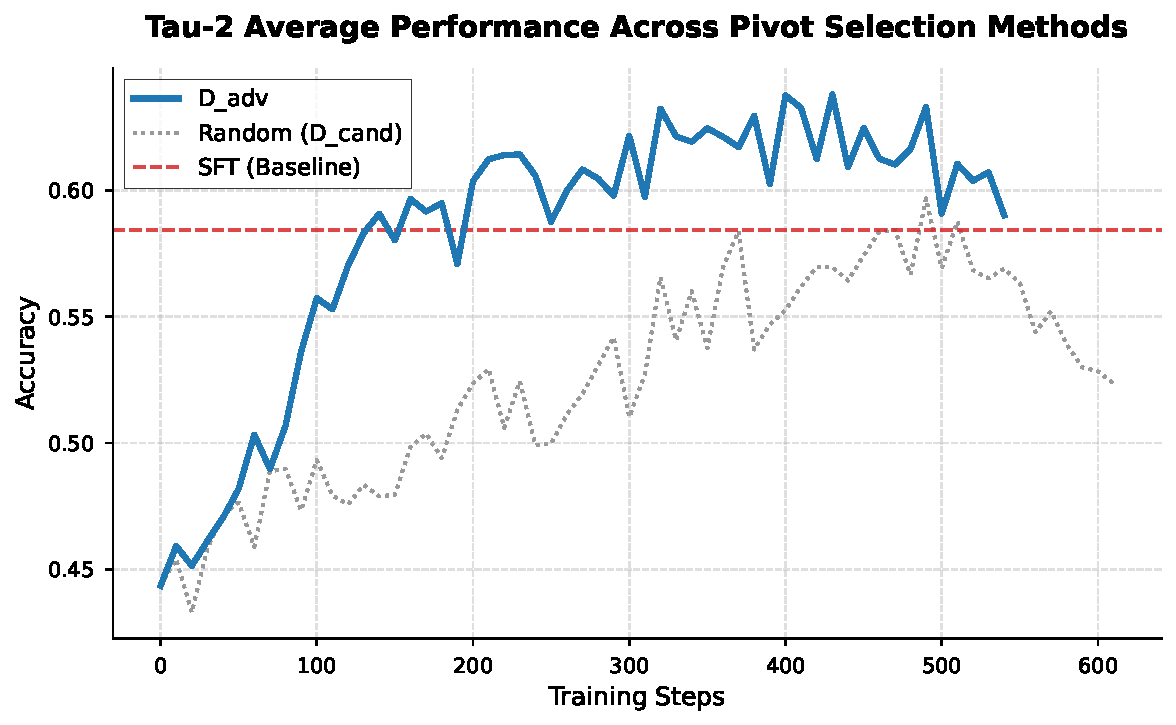
\includegraphics[width=0.5\textwidth]{figures/main_average_validation.pdf}
%     \caption{$\tau^2$-bench performance throughout RL training. Choosing pivots with a large advantage gap yields superior model improvement compared to choosing pivots with nonzero advantage or randomly choosing pivots.}
%     \label{fig:rl_tau_pivot_selection_acc}

%     \centering
%     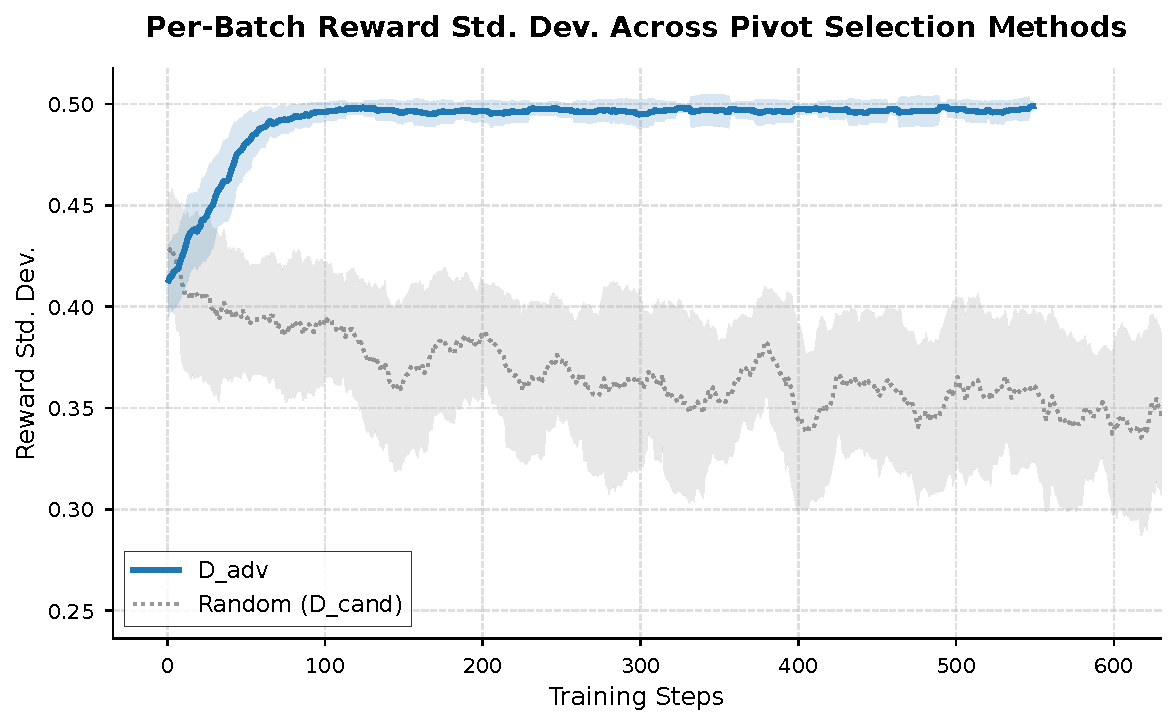
\includegraphics[width=0.5\textwidth]{figures/tau_reward_stddev.pdf}
%     \caption{$\tau^2$-bench training reward standard deviation over training. The random reward setting quickly yields unbalanced training rewards while the mixed rewards and high advantage gap settings leads to higher standard deviation in training rewards per group, allowing for better GRPO training.}
%     \label{fig:rl_tau_pivot_selection_acc}
% \end{figure}
\begin{figure}[t]
    \centering
    % Left side minipage
    \begin{minipage}{0.48\textwidth}
        \centering
        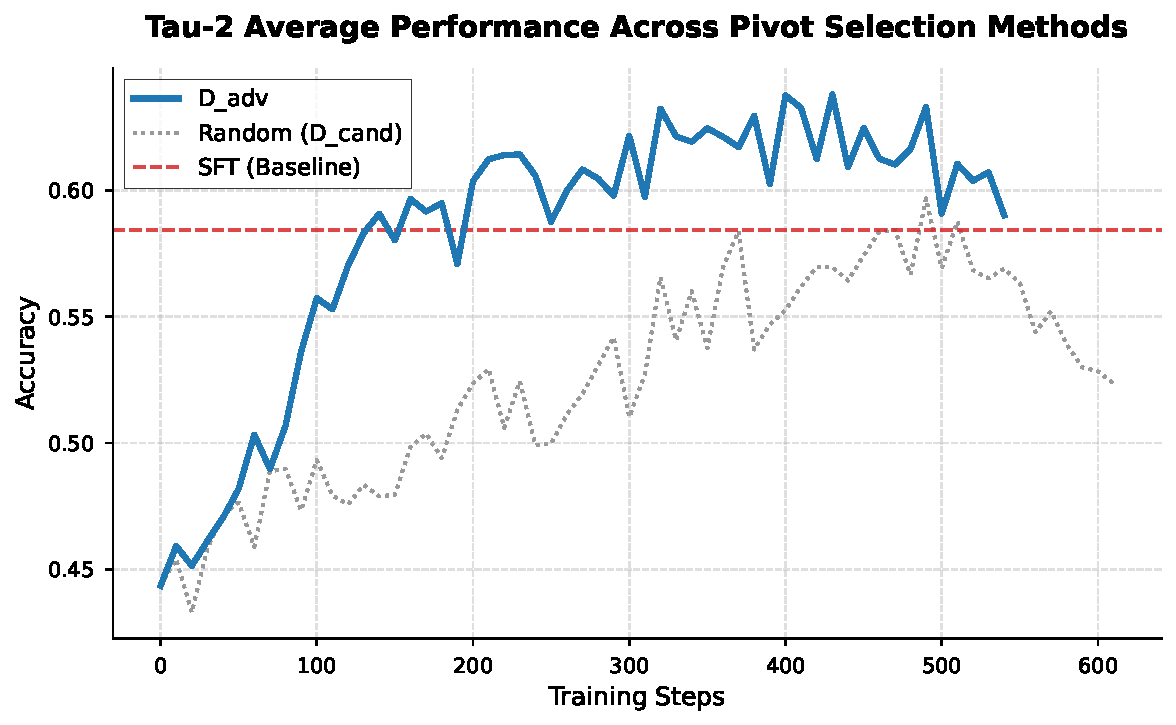
\includegraphics[width=\linewidth]{figures/main_average_validation.pdf}
        \caption{$\tau^2$-bench performance throughout RL training. Choosing pivots with a large advantage gap yields superior model improvement, outperforming even SFT on the base dataset.}
        \label{fig:rl_tau_pivot_selection_acc}
    \end{minipage}
    \hfill % Adds horizontal space between the two minipages
    % Right side minipage
    \begin{minipage}{0.48\textwidth}
        \centering
        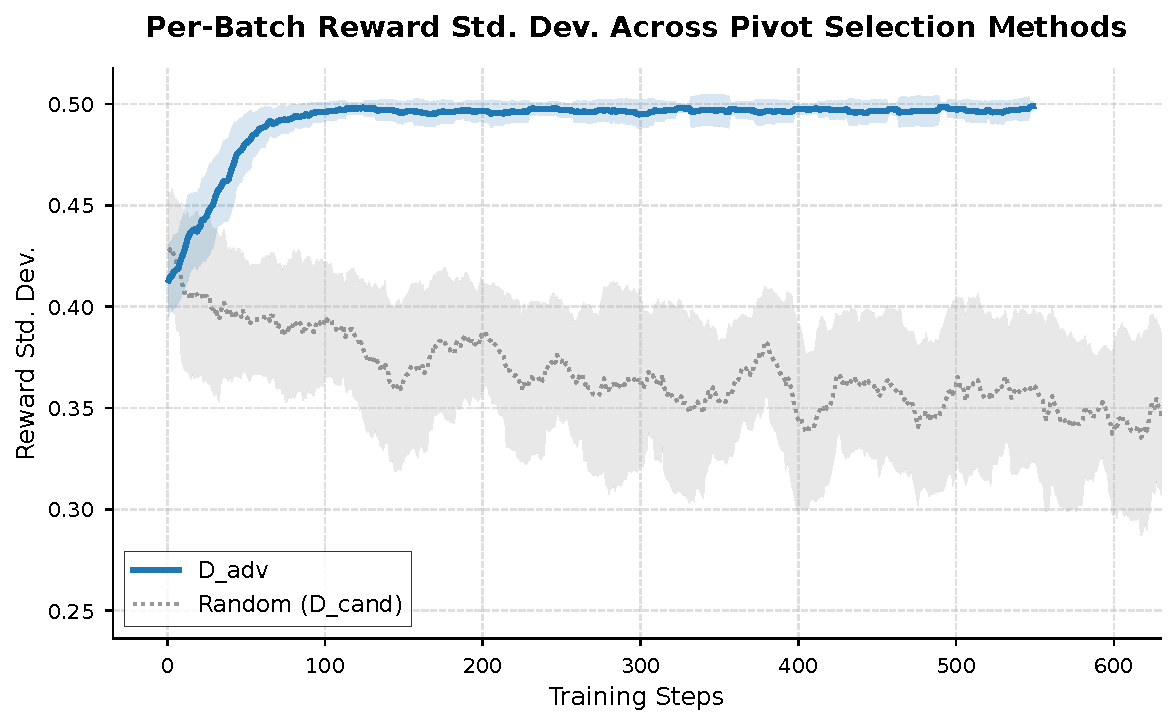
\includegraphics[width=\linewidth]{figures/tau_reward_stddev.pdf}
        \caption{$\tau^2$-bench training reward standard deviation. Higher standard deviation in training rewards allows for better GRPO training. Showing rolling standard deviation for viewer readability.}
        \label{fig:rl_tau_reward_stddev}
    \end{minipage}
\end{figure}

\begin{figure*}[t]
    \centering
    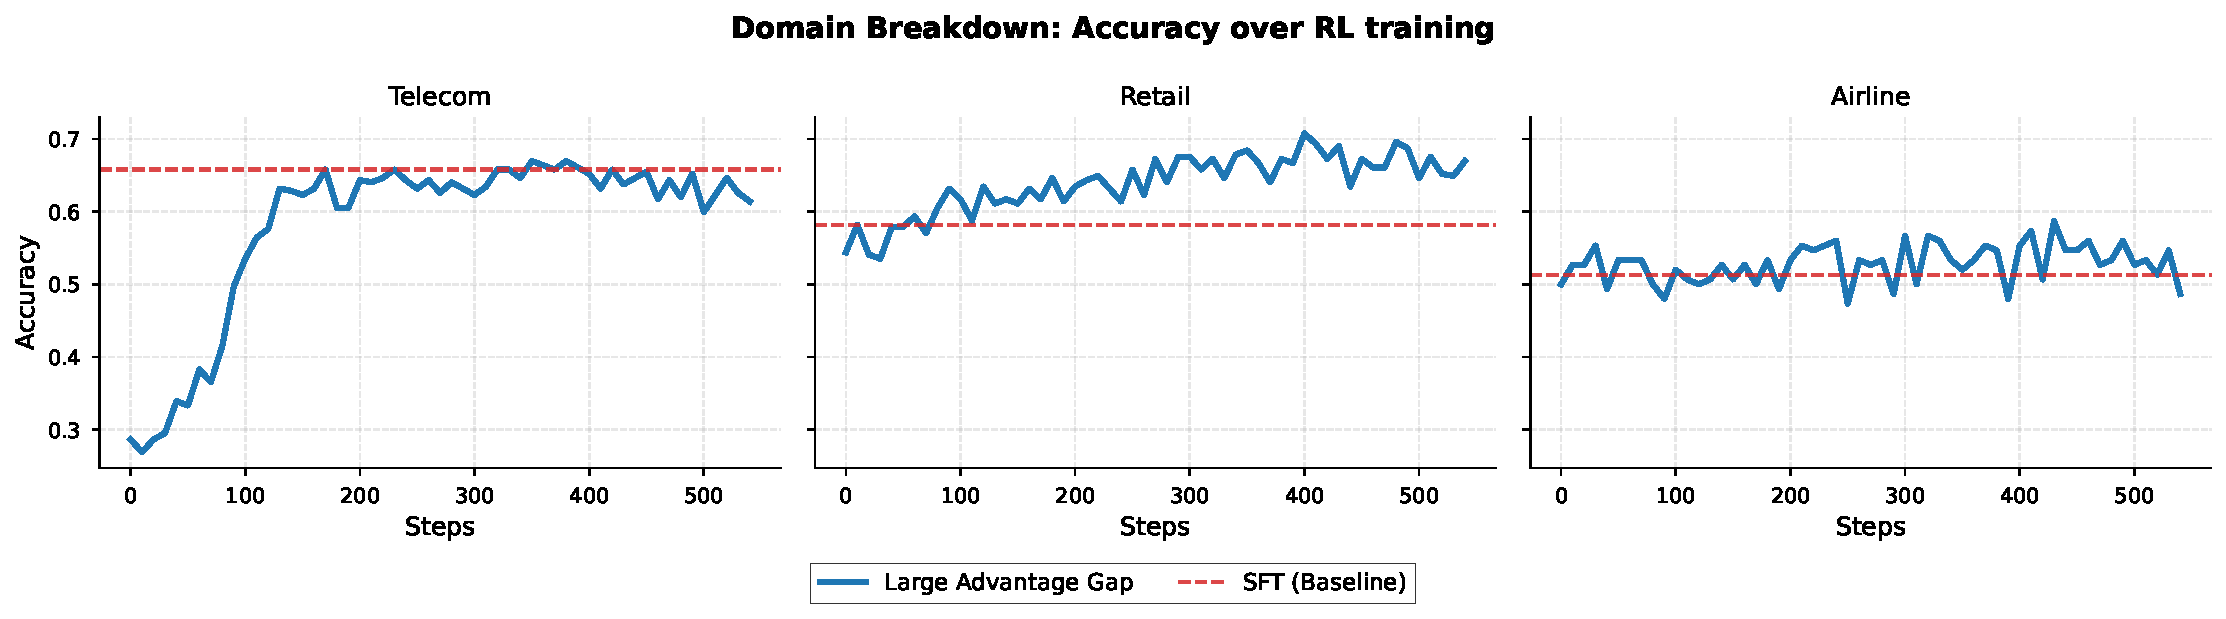
\includegraphics[width=1.0\textwidth]{figures/main_per_domain_validation_difficulty.pdf}
    \caption{Per-domain benchmark performance over RL training. From left to right: Telecom, Retail, Airline.}
    \label{fig:rl_domain}
\end{figure*}


\subsubsection{Effect of Pivot Selection}
In Figures \ref{fig:rl_tau_pivot_selection_acc} and \ref{fig:rl_tau_reward_stddev}, we observe the effect of different pivot selection algorithms by the change in accuracy over RL training steps as well as the training reward standard deviation over RL steps. While the random pivot selection baseline is able to improve the model, it under-performs the mixed rewards setting where at the beginning of training every input prompt has non-zero advantage. Empirically, this is shown as the standard deviation of the reward for that prompt across the rollouts being larger. Meanwhile, further constraining the dataset to choose from points where the advantage gap is large yields the best performing training dataset, improving the model accuracy from $44.35\%$ to $63.81\%$ after 430 steps of training. We also see that as training goes, the large advantage gap set also has a more balanced reward distribution for each prompt as can be seen with the higher training reward standard deviation.



\subsection{Terminal-Bench}
\subsubsection{Experimental Details}
We collected resolved and completed trajectories from \texttt{Qwen/Qwen3-Coder-480B-A35B-Instruct} and \texttt{moonshotai/Kimi-K2-Instruct} on Terminal Bench using the Terminus 1 and Terminus 2 agents, and use all assistant bash actions as pivots. From the $\mathcal{D}_{\text{adv}}$ setting, we additionally deduplicate similar commands to achieve diversity in the data. Our final training set consisted of approximately 20,000 samples. For verification in the RL environment, we employed output schema validation, string similarity, and equivalency-based LLM-as-judge in the reward design.

\subsection{SWE-Bench Verified}
\subsubsection{Experimental Details}
We use an internal dataset of trajectories generated using the OpenHands \citep{wang2025openhandsopenplatformai}, OpenCode \citep{opencode}, and Codex \citep{openaicodex_software} harnesses on tasks including SWE-Gym \citep{pan2025trainingsoftwareengineeringagents}, and R2E-Gym \citep{jain2025r2egymproceduralenvironmentshybrid} using the \texttt{MiniMaxAI/MiniMax-M2.5} \citep{minimax2026m25} model. We evaluate the mean@3 score using the OpenHands harness. To create the PivotRL dataset, we use all tool call actions that did not result in error calls as pivots, and use a string similarity verifier that matches only tool call names for $r_{\name}$. We curate a final dataset in the $\mathcal{D}_{\text{adv}}$ setting of size $87718$ for training.


\subsection{BrowseComp}
\subsubsection{Experimental Details}
We start with a multi-hop question-answer dataset and use an online search engine along with \texttt{DeepSeek-V3.2} to generate trajectories from it. We curate a set of $13215$ samples and use random filtering ($\mathcal{D}_{\text{random}}$) due to the small size of the dataset. We use this dataset to train on top of \texttt{Qwen3-30B-A3B-Thinking-2507}.
\subsubsection{Results}
Under the best settings, we are able to improve \texttt{Qwen3-30B-A3B-Thinking-2507} from $2.5$ accuracy to $11.3$.


\begin{table*}[!t]
\centering
\small
\begin{tabular}{l c cc c}
\toprule
\multirow{2}{*}{\textbf{Benchmark}} 
& \multirow{2}{*}{\textbf{Baseline}} 
& \multicolumn{2}{c}{\textbf{Multi-Domain Training}}
& \multirow{2}{*}{\textbf{RL vs SFT ($\Delta$)}} \\
\cmidrule(lr){3-4}
& Qwen3-30B 
& \textbf{SFT} & \textbf{RL} & \\
\midrule
\midrule

\multicolumn{5}{l}{\textit{In-Domain Benchmarks}} \\
\midrule

Tau2 
& 44.35 
& 57.60 (+13.25) & 56.33 (+11.98) 
& -1.27 \\

SWE-Verified
& 19.07 
& -- \quad (--) & 32.87 (+13.80) 
& -- \\

Terminal-Bench
& 5.42 
& -- \quad (--) & -- \quad (--) 
& -- \\

BrowseComp
& 2.50 
& -- \quad (--) & -- \quad (--) 
& -- \\

\midrule
\multicolumn{5}{l}{\textit{Out-of-Domain Benchmarks}} \\
\midrule

IFBench 
& 52.04 
& 47.71 (-4.33)  & 50.41 (-1.63) 
& +2.70 \\

AIME25 
& 86.04 
& 83.13 (-2.91)  & 85.83 (-0.21) 
& +2.70 \\

MATH500 
& 98.05 
& 98.15 (+0.10)  & 98.15 (+0.10) 
& 0.00 \\

LiveCodeBench 
& 66.52 
& 60.57 (-5.95)  & 67.40 (+0.88) 
& +6.83 \\

Scicode 
& 36.83 
& 26.18 (-10.65) & 38.17 (+1.34) 
& +11.99 \\

MMLU-Pro 
& 80.84 
& 80.97 (+0.13)  & 81.14 (+0.30) 
& +0.17 \\

MMLU-ProX 
& 78.58 
& -- \quad (--)  & 78.74 (+0.16) 
& -- \\

WMT24++ 
& 36.97 
& 34.87 (-2.10)  & 36.92 (-0.05) 
& +2.05 \\

\bottomrule
\end{tabular}
\caption{Evaluation results for Multi-domain training.}
\label{tab:combined_training_results}
\end{table*}

\subsection{Multi-domain Training}
\subsubsection{Experimental Setup}
We additionally train a model on all domains combined. For SFT, we combine all 4 SFT datasets using temperature sampling with $\text{temperate}=0.5$, which yields a dataset that is: conversational tool-use: 56.38\%), (swe: 11.01\%), (terminal: 31.36\%), and (search: 1.25\%). We conduct training with batch size 128 and learning rate 5e-6. For \name, we combine the 4 RL datasets with equal weighing. Using batch size 128, each domain will have an average of 32 groups per batch. We rollout 16 times per prompt with a 1e-6 learning rate with one gradient update per batch.

\subsubsection{Results and Analysis}
The evaluation results of resulting models are shown in Table \ref{tab:combined_training_results}. For in-domain benchmarks, PivotRL is competitive to SFT. In out of domain benchmarks, PivotRL is significantly better at retaining existing capabilities compared to SFT. The results clearly show that PivotRL can be adopted as a general training framework for improving the capabilities of models in multiple domains simultaneously without significant concern for catastrophic forgetting.

